% Options for packages loaded elsewhere
\PassOptionsToPackage{unicode}{hyperref}
\PassOptionsToPackage{hyphens}{url}
%
\documentclass[
  letterpaper,
]{book}

\usepackage{amsmath,amssymb}
\usepackage{lmodern}
\usepackage{iftex}
\ifPDFTeX
  \usepackage[T1]{fontenc}
  \usepackage[utf8]{inputenc}
  \usepackage{textcomp} % provide euro and other symbols
\else % if luatex or xetex
  \usepackage{unicode-math}
  \defaultfontfeatures{Scale=MatchLowercase}
  \defaultfontfeatures[\rmfamily]{Ligatures=TeX,Scale=1}
\fi
% Use upquote if available, for straight quotes in verbatim environments
\IfFileExists{upquote.sty}{\usepackage{upquote}}{}
\IfFileExists{microtype.sty}{% use microtype if available
  \usepackage[]{microtype}
  \UseMicrotypeSet[protrusion]{basicmath} % disable protrusion for tt fonts
}{}
\makeatletter
\@ifundefined{KOMAClassName}{% if non-KOMA class
  \IfFileExists{parskip.sty}{%
    \usepackage{parskip}
  }{% else
    \setlength{\parindent}{0pt}
    \setlength{\parskip}{6pt plus 2pt minus 1pt}}
}{% if KOMA class
  \KOMAoptions{parskip=half}}
\makeatother
\usepackage{xcolor}
\setlength{\emergencystretch}{3em} % prevent overfull lines
\setcounter{secnumdepth}{5}
% Make \paragraph and \subparagraph free-standing
\ifx\paragraph\undefined\else
  \let\oldparagraph\paragraph
  \renewcommand{\paragraph}[1]{\oldparagraph{#1}\mbox{}}
\fi
\ifx\subparagraph\undefined\else
  \let\oldsubparagraph\subparagraph
  \renewcommand{\subparagraph}[1]{\oldsubparagraph{#1}\mbox{}}
\fi


\providecommand{\tightlist}{%
  \setlength{\itemsep}{0pt}\setlength{\parskip}{0pt}}\usepackage{longtable,booktabs,array}
\usepackage{calc} % for calculating minipage widths
% Correct order of tables after \paragraph or \subparagraph
\usepackage{etoolbox}
\makeatletter
\patchcmd\longtable{\par}{\if@noskipsec\mbox{}\fi\par}{}{}
\makeatother
% Allow footnotes in longtable head/foot
\IfFileExists{footnotehyper.sty}{\usepackage{footnotehyper}}{\usepackage{footnote}}
\makesavenoteenv{longtable}
\usepackage{graphicx}
\makeatletter
\def\maxwidth{\ifdim\Gin@nat@width>\linewidth\linewidth\else\Gin@nat@width\fi}
\def\maxheight{\ifdim\Gin@nat@height>\textheight\textheight\else\Gin@nat@height\fi}
\makeatother
% Scale images if necessary, so that they will not overflow the page
% margins by default, and it is still possible to overwrite the defaults
% using explicit options in \includegraphics[width, height, ...]{}
\setkeys{Gin}{width=\maxwidth,height=\maxheight,keepaspectratio}
% Set default figure placement to htbp
\makeatletter
\def\fps@figure{htbp}
\makeatother
\newlength{\cslhangindent}
\setlength{\cslhangindent}{1.5em}
\newlength{\csllabelwidth}
\setlength{\csllabelwidth}{3em}
\newlength{\cslentryspacingunit} % times entry-spacing
\setlength{\cslentryspacingunit}{\parskip}
\newenvironment{CSLReferences}[2] % #1 hanging-ident, #2 entry spacing
 {% don't indent paragraphs
  \setlength{\parindent}{0pt}
  % turn on hanging indent if param 1 is 1
  \ifodd #1
  \let\oldpar\par
  \def\par{\hangindent=\cslhangindent\oldpar}
  \fi
  % set entry spacing
  \setlength{\parskip}{#2\cslentryspacingunit}
 }%
 {}
\usepackage{calc}
\newcommand{\CSLBlock}[1]{#1\hfill\break}
\newcommand{\CSLLeftMargin}[1]{\parbox[t]{\csllabelwidth}{#1}}
\newcommand{\CSLRightInline}[1]{\parbox[t]{\linewidth - \csllabelwidth}{#1}\break}
\newcommand{\CSLIndent}[1]{\hspace{\cslhangindent}#1}

\makeatletter
\makeatother
\makeatletter
\@ifpackageloaded{bookmark}{}{\usepackage{bookmark}}
\makeatother
\makeatletter
\@ifpackageloaded{caption}{}{\usepackage{caption}}
\AtBeginDocument{%
\ifdefined\contentsname
  \renewcommand*\contentsname{Table of contents}
\else
  \newcommand\contentsname{Table of contents}
\fi
\ifdefined\listfigurename
  \renewcommand*\listfigurename{List of Figures}
\else
  \newcommand\listfigurename{List of Figures}
\fi
\ifdefined\listtablename
  \renewcommand*\listtablename{List of Tables}
\else
  \newcommand\listtablename{List of Tables}
\fi
\ifdefined\figurename
  \renewcommand*\figurename{Figure}
\else
  \newcommand\figurename{Figure}
\fi
\ifdefined\tablename
  \renewcommand*\tablename{Table}
\else
  \newcommand\tablename{Table}
\fi
}
\@ifpackageloaded{float}{}{\usepackage{float}}
\floatstyle{ruled}
\@ifundefined{c@chapter}{\newfloat{codelisting}{h}{lop}}{\newfloat{codelisting}{h}{lop}[chapter]}
\floatname{codelisting}{Listing}
\newcommand*\listoflistings{\listof{codelisting}{List of Listings}}
\makeatother
\makeatletter
\@ifpackageloaded{caption}{}{\usepackage{caption}}
\@ifpackageloaded{subcaption}{}{\usepackage{subcaption}}
\makeatother
\makeatletter
\@ifpackageloaded{tcolorbox}{}{\usepackage[many]{tcolorbox}}
\makeatother
\makeatletter
\@ifundefined{shadecolor}{\definecolor{shadecolor}{rgb}{.97, .97, .97}}
\makeatother
\makeatletter
\makeatother
\ifLuaTeX
  \usepackage{selnolig}  % disable illegal ligatures
\fi
\IfFileExists{bookmark.sty}{\usepackage{bookmark}}{\usepackage{hyperref}}
\IfFileExists{xurl.sty}{\usepackage{xurl}}{} % add URL line breaks if available
\urlstyle{same} % disable monospaced font for URLs
\hypersetup{
  pdftitle={Introduction to Digital History},
  pdfauthor={Ina Serif},
  hidelinks,
  pdfcreator={LaTeX via pandoc}}

\title{Introduction to Digital History}
\author{Ina Serif}
\date{}

\begin{document}
\frontmatter
\maketitle
\ifdefined\Shaded\renewenvironment{Shaded}{\begin{tcolorbox}[boxrule=0pt, enhanced, interior hidden, frame hidden, breakable, borderline west={3pt}{0pt}{shadecolor}, sharp corners]}{\end{tcolorbox}}\fi

\renewcommand*\contentsname{Table of contents}
{
\setcounter{tocdepth}{2}
\tableofcontents
}
\mainmatter
\bookmarksetup{startatroot}

\hypertarget{welcome}{%
\chapter*{Welcome}\label{welcome}}
\addcontentsline{toc}{chapter}{Welcome}

\markboth{Welcome}{Welcome}

Der vorliegende Guide begleitet die Einführungskurse im Fach Geschichte
an der Universität Basel und soll einen ersten Einblick in den Bereich
digital history geben. Die epochen- und areaspezifischen Inhalte der
verschiedenen Einführungskurse sollen dabei berücksichtigt werden, die
Verweise auf verschiedene digital-history-Projekte aus unterschiedlichen
Epochen mit der Zeit also anwachsen.

Der Guide wird für die Teilnehmer:innen der Einführungskurse von einer
Präsenzsitzung begleitet, bietet aber hoffentlich auch unabhängig davon
einen Mehrwert. Für Kommentare, Anregungen oder Beschwerden freue ich
mich über eine Nachricht.

Der Guide ist in zwei Teile gegliedert: Die Kapitel 1--5 sollen eine
erste Übersicht über ``digital history'' bieten und den Blick auf
Neuerungen und Veränderungen richten, die sich in den
Geschichtswissenschaften aus der Nutzung digitaler Methoden ergeben. Der
anschließende Praxisteil zeigt an einem konkreten Beispiel die Anwendung
verschiedener Techniken auf, die sich (nicht nur) für Historiker:innen
bei der Arbeit mit Quellenmaterial anbieten. Der Praxisteil verfolgt
dabei zwei Ziele: Zum einen sollen Hemmungen bei der Arbeit mit dem
Computer, die über die Nutzung als elektronische Schreibmaschine
hinausgeht, abgebaut werden. Zum zweiten sollen ein grundlegendes
Verständnis dafür hergestellt werden, welche Möglichkeiten
computergestützte Analysen bieten und wie diese in der historischen
Arbeit eingesetzt werden können.

Die Übersicht soll möglichst knapp gehalten werden -- es gibt zahlreiche
ausführliche Grundlagenwerke, weswegen viele Themen nur kurz
angeschnitten, dafür aber mit weiterführenden Verweisen versehen werden.
Dasselbe gilt für den Praxisteil: Weiterreichende Anleitungen, Tutorials
oder Onlinekurse werden an entsprechender Stelle verlinkt.
Vollständigkeit wird an keiner Stelle beansprucht; Hinweise auf weitere
Online-Angebote nehme ich gerne auf.

\bookmarksetup{startatroot}

\hypertarget{was-ist-digital-history}{%
\chapter{Was ist digital history?}\label{was-ist-digital-history}}

Über die Antwort zur Frage, was digital history ist oder umfasst, kann
man ausgiebig diskutieren; als Teilgebiet der digital humanities, der
digitalen Geisteswissenschaften, kann die folgende aktuelle und
pragmatische Definition von Blaney et al.~hilfreich sein:

\begin{quote}
Digital humanities, in our view, is a question of approach: if you are
actively and critically using digital tools to aid your work in
researching, teaching or learning, you are probably doing digital
humanities. We would encourage anyone to learn to program if they are
interested in doing so, but we do not see it as a defining
characteristic of work in digital humanities.\footnote{Blaney, Jonathan;
  Winters, Jane; Milligan, Sarah u.~a.: Doing digital history: a
  beginner's guide to working with text as data, Manchester 2021 ({IHR}
  research guides), S.~6.}
\end{quote}

Dabei umfassen ``digital tools'' eine große Bandbreite -- und es wird
sich kaum eine:r finden, der:die Studium, Forschung oder Lehre völlig
ohne die Nutzung digitaler Techniken betreibt. Wir sind alle
Historiker:innen im digitalen Zeitalter, und als solche müssen wir
ohnehin neue Kompetenzen entwickeln. Wir können uns aber zudem dafür
entscheiden, für ein Forschungsprojekt Methoden und Techniken
einzusetzen, die über die traditionellen Werkzeuge der
Geschichtswissenschaften hinausgehen -- Analyse und Interpretation von
Quellen durch deren genaue Lektüre, sogenanntes \emph{close reading} --,
und uns durch den Computer unterstützen lassen. Ob wir hierbei auf
vorhandene Software zurückgreifen oder selbst Programme schreiben, um
uns nicht nur als Historiker:innen im digitalen Zeitalter, sondern auch
als digitale Historiker:innen zu verstehen, mögen manche als
Glaubensfrage auffassen; eine inkludierende Haltung zu dieser Frage
scheint mir dabei nur Vorteile zu haben.\footnote{Entgegen einer häufig
  zitierten Aussage von Emmanuel Le Roy Ladurie (*1929), der Historiker
  von morgen werde Programmierer sein, oder er werde nicht sein:
  ``L'historien de demain sera programmeur ou il ne sera pas.'' Le Roy
  Ladurie, Emmanuel: La fin des {é}rudits, in: Le Nouvel Observateur,
  08.1968.}

Für eine erste Idee dafür, wie man historische Fragestellungen mithilfe
digitaler Methoden beantworten kann und wie unterschiedlich digital
unterstützte Forschungsprojekte aussehen können, bietet sich unter
anderem der Übersichtsartikel
``\href{https://onlinelibrary.wiley.com/doi/10.1111/1468-229X.12969}{State
of the Field: Digital History}'' von Romein et al.~(2020) an.\footnote{Romein,
  C. Annemieke; Kemman, Max; Birkholz, Julie M. u.~a.: State of the
  {Field}: {Digital} {History}, in: History 105~(365), 04.2020,
  S.~291--312. Online:
  \textless{}\url{https://doi.org/10.1111/1468-229X.12969}\textgreater,
  Stand: 15.09.2022.} Eine anwachsende Liste an Beispielprojekten aus
unterschiedlichen Epochen bzw. Themenbereichen findet sich in
Section~\ref{sec-projects}.

Um eine Annäherung an die aktive, kritische und reflektierte Nutzung
digitaler Methoden in Forschung und Lehre mit einem Fokus auf deren
Anwendung in den Geschichtswissenschaften geht es im vorliegenden Guide.
Weiterführende Texte zur Frage, was digital history ist bzw. umfasst,
finden sich in \textbf{?@sec-digitalhistory-paper}.

\bookmarksetup{startatroot}

\hypertarget{forschung-und-lehre}{%
\chapter{Forschung und Lehre}\label{forschung-und-lehre}}

Die fortschreitende Digitalisierung vorhandener Quellen
(Retrodigitalisierung) und die unaufhörliche Entstehung neuer Quellen im
digitalen Raum (born digital data) beeinflusst zunehmend unsere Arbeit
als Historiker:innen.

\begin{figure}

\href{history_department}{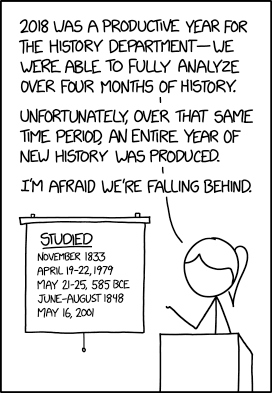
\includegraphics{https://imgs.xkcd.com/comics/history_department.png}}

\caption{Randall Munroe, History Department, xkcd.com (17.12.2018).
``When we take into account the recent discovery of previously-unstudied
history in the 1750s, this year may have been an outright loss.''}

\end{figure}

Veränderungen und Entwicklungen betreffen dabei unterschiedliche Ebenen,
auf die im Folgenden kurz eingegangen wird: die Existenz bzw. der Umgang
mit digitalen/digitalisierten Quellen,

\hypertarget{digitale-tools-zur-kommunikation}{%
\section{Digitale Tools zur
Kommunikation}\label{digitale-tools-zur-kommunikation}}

\hypertarget{digitale-tools-zur-analyse}{%
\section{Digitale Tools zur Analyse}\label{digitale-tools-zur-analyse}}

\hypertarget{digitale-elemente-in-der-hochschullehre}{%
\section{Digitale Elemente in der
Hochschullehre}\label{digitale-elemente-in-der-hochschullehre}}

\hypertarget{sec-projects}{%
\section{Projekte und Ressourcen}\label{sec-projects}}

\hypertarget{alte-geschichte}{%
\subsection{Alte Geschichte}\label{alte-geschichte}}

\hypertarget{mittelalter-und-fruxfche-neuzeit}{%
\subsection{Mittelalter und Frühe
Neuzeit}\label{mittelalter-und-fruxfche-neuzeit}}

\hypertarget{moderne-und-zeitgeschichte}{%
\subsection{Moderne und
Zeitgeschichte}\label{moderne-und-zeitgeschichte}}

\hypertarget{juxfcdische-geschichte}{%
\subsection{Jüdische Geschichte}\label{juxfcdische-geschichte}}

\begin{itemize}
\item
  \href{https://jewishstudies.washington.edu/digital-jewish-studies/}{Digital
  Jewish Studies Online}, Stroum Center for Jewish Studies, University
  of Washington
\item
  Menny, Anna; Rürup, Miriam; Siegel, Björn: Jüdische Geschichte im
  deutschsprachigen Raum, in: Busse, Laura u.~a.~(Hg.): Clio-Guide. Ein
  Handbuch zu digitalen Ressourcen für die Geschichtswissenschaften,
  Berlin 2018, S. E.2-1--E.2-56. Online:
  \url{https://doi.org/10.18452/19244}.
\end{itemize}

\hypertarget{geschichte-afrikas}{%
\subsection{Geschichte Afrikas}\label{geschichte-afrikas}}

\hypertarget{osteuropuxe4ische-geschichte}{%
\subsection{Osteuropäische
Geschichte}\label{osteuropuxe4ische-geschichte}}

\bookmarksetup{startatroot}

\hypertarget{shell}{%
\chapter{shell}\label{shell}}

Shell 101

Es gibt zwei Arten, um mit dem Computer zu interagieren bzw. ihn zu
nutzen: über ein \textbf{G}raphical \textbf{U}ser \textbf{I}nterface
(GUI) oder, etwas direkter, über die
\href{https://de.wikipedia.org/wiki/Kommandozeile}{Kommandozeile}\footnote{Kommandozeile/command
  line, bash, shell, prompt finden sich oft als synonym genutzte
  Begriffe für Command Line Interfaces. Auf UNIX-basierten
  Betriebssystemen wie Mac OS und Linux ist das Terminal als Interface
  weit verbreitet; für Details:
  https://en.wikipedia.org/wiki/Command-line\_interface\#History.
  Windowsnutzer:innen kommen mit der Powershell ganz gut zurecht, es
  empfiehlt sich eventuell die Installation von
  \href{https://en.wikipedia.org/wiki/Cygwin}{Cygwin} oder
  \href{https://en.wikipedia.org/wiki/MinGW}{MinGW}, um mit einem
  UNIX-basierten Interface arbeiten zu können.}. Um eine Datei
``Bild1.jpg'' im Ordner ``Bilder'' zu löschen, öffnet man den Explorer
(Windows) oder den Finder (Mac), klickt sich zum Ordner ``Bilder'',
macht einen Rechtsklick auf die zu löschende Datei ``Bild1.jpg'', klickt
``In den Papierkorb legen'' oder zieht die Datei mit der Maus direkt
dorthin. Man kann dieselbe Aktion als Kommando eintippen: Man öffnet
eine Powershell (Windows) oder das Terminal (Mac), navigiert mit
Texteingabe zum entsprechenden Ordner, bspw.
\texttt{cd\ Dokumente/Bilder} und gibt dort das Kommando
\texttt{rm\ "Datei.jpg"} ein, das mit der Entertaste ausgeführt wird.

\texttt{(base)\ serina00@dg-19-mac-02\ Bilder\ \%\ rm\ "Datei.jpg"}

Die beiden Vorgehensweisen unterscheiden sich dabei in drei Punkten:

\begin{enumerate}
\def\labelenumi{\arabic{enumi}.}
\tightlist
\item
  Das Kommando \texttt{rm} ist endgültig, die Datei ist ohne
  Übergangszeit im Papierkorb gelöscht.
\item
  Das Kommando lässt sich relativ simpel auf eine Vielzahl von
  Dokumenten anwenden, wobei ganz unterschiedliche Bedingungen beachtet
  werden können, und es lässt sich mit anderen Kommandos verbinden.
\item
  Terminal sieht k3wl aus.
\end{enumerate}

Bevor wir den zweiten -- und für unsere Arbeit hilfreichsten --
Unterschied genauer anschauen, kurz zur Kommandozeile:

In einem Terminal/Shell können Befehle/Programme ausgeführt werden, die
auf der Datenstrukturebene stattfinden -- wie beispielsweise das Löschen
einer Datei, \texttt{rm\ Dateiname.xyz}, oder das Erstellen eines
Ordners, \texttt{mkdir\ NeuerOrdner}. Oder aber Operationen auf
Dateninhaltsebene -- wie beispielsweise das Suchen eines bestimmten
Begriffs in einer Textdatei, \texttt{grep\ Begriff\ Textdatei.txt}, oder
das Auszählen mehrerer Begriffe und das Speichern des Ergebnisses in
einer neuen Datei,
\texttt{grep\ -Ec\ "Begriff1\textbar{}Begriff2"\ Textdatei.txt\ \textgreater{}\ Ergebnisse.txt}.

Woher weiss Ihre Shell aber, was sie ausführen soll, wenn Sie
\texttt{rm} oder \texttt{grep} eintippen? Es gibt zahlreiche
Shell-Programme, die bereits auf Ihrem System vorinstalliert sind, und
mit denen Sie vieles tun können -- öffnen Sie Ihre Shell und tippen Sie
\texttt{date} ein: Das aktuelle Datum mit Uhrzeit erscheint. Ihre Shell
sucht nach dem ersten Argument, dem Befehl, im Filesystem des Computers,
und wenn sie fündig wird, führt sie eine Aktion mit den entsprechenden
Parametern aus.

\begin{quote}
tmi: Wenn Sie \texttt{echo\ \$PATH} im Terminal eingeben, sehen Sie eine
Auflistung der Orte, an denen nach Befehlen gesucht wird. Tippen Sie
\texttt{which\ date} ein und drücken Sie `Enter', um zu sehen, wo das
Programm ``date'' in Ihrem Computer liegt.
\end{quote}

Wenn Sie einen Befehl eintippen, den es nicht gibt bzw. für den es noch
kein installiertes Programm auf Ihrem Computer gibt, bekommen Sie eine
simple Fehlermeldung:

\texttt{(base)\ serina00@dg-19-mac-02\ EK-dh\ \%\ nonsense}

\texttt{command\ not\ found:\ nonsense}

Das aktuelle Datum wird Ihnen wahrscheinlich auch in Ihrer Toolbar
angezeigt, und einen neuen Ordner können Sie per Rechtsklick erstellen,
dazu brauchen Sie das Terminal nicht unbedingt. Um einen Begriff in
einem Textdokument zu finden und alle Vorkommen zu zählen, können Sie
das Dokument öffnen, \texttt{Strg-F} drücken, den Begriff eingeben und
das Ergebnis sehen. Wenn Sie nach mehreren Begriffen suchen wollen,
müssen Sie dieselbe Aktion zweimal ausführen: \texttt{Strg-F}, Begriff
2.

Wenn Sie wissen möchten, wie häufig Arthur Dent, Zaphod Beeblebrox,
Slartibartfast und Mrs Enid Kapelsen in den sechs Bänden von
``\href{https://en.wikipedia.org/wiki/The_Hitchhiker\%27s_Guide_to_the_Galaxy}{The
Hitchhiker's Guide to the Galaxy}'' genannt werden, müssen Sie, wenn Sie
den
\href{https://archive.org/stream/TheultimateHitchhikersGuide/The\%20Hitchhiker\%27s\%20Guide\%20To\%20The\%20Galaxy_djvu.txt}{Volltext}
heruntergeladen haben, für jeden Namen eine Suche ausführen, mit
\texttt{Strg-F}. Bei der Suche nach Personen mit Vor- und Nachnamen wie
``Arthur Dent'' suchen Sie nach ``Arthur'', nach ``Dent'' und nach
``Arthur Dent'' und ziehen alle ``Arthur Dent''-Treffer von den übrigen
Treffern ab, um nichts doppelt zu zählen und ihre Suchergebnisse zu
verfälschen. Die Trefferzahl all Ihrer Suchanfragen schreiben Sie in ein
neues Dokument.

Sie können dasselbe auch mit dem Terminal machen und einige der
Built-in-Programme nutzen: Sie bewegen sich mit \texttt{cd},
\texttt{change\ directory}, in den Ordner (directory), in dem Ihre
Textdatei liegt:

\texttt{(base)\ serina00@dg-19-mac-02\ serina00\ \%\ cd\ Documents/progr/EK\_dh/Hitchhiker}

(Um zu prüfen, was dort liegt, können Sie im Terminal \texttt{ls} (für
\texttt{list}) eingeben, bzw. in der Powershell \texttt{dir} (für
\texttt{directory})

\texttt{(base)\ serina00@dg-19-mac-02\ Hitchhiker\ \%\ ls\ hitchhiker\_fulltext}

Mit einer Zeile können Sie die in einem Texteditor ausgeführten
Suchvorgänge mit \texttt{grep} (Global Regular Expression Print)
ausführen und die Ergebnisse mit \texttt{\textgreater{}} in eine neue
Datei schreiben:

\appendix
\addcontentsline{toc}{part}{Appendices}

\hypertarget{appendix}{%
\chapter{Appendix}\label{appendix}}

\begin{longtable}[]{@{}
  >{\raggedright\arraybackslash}p{(\columnwidth - 2\tabcolsep) * \real{0.1058}}
  >{\raggedright\arraybackslash}p{(\columnwidth - 2\tabcolsep) * \real{0.8942}}@{}}
\toprule()
\endhead
API & \textbf{A}pplication \textbf{P}rogramming \textbf{I}nterface: a
facility offered by a web resource which allows search queries
independent of a \textbf{GUI}, often performed using scripts \\
bash & default program that runs in the \textbf{command line} \\
big data & huge amount of data, identifiable through repeated freezing
of your standard program when opening a file \\
born digital data & data which originated in a digital form \\
CLI & \textbf{C}ommand \textbf{L}ine \textbf{I}nterface, text interface
that allows interaction with the computer; see also \textbf{bash} \\
CMS & \textbf{C}ontent \textbf{M}anagement \textbf{S}ystem \\
Console & See \textbf{CLI} \\
Crowdsourcing & projects that include the active participation of the
public to generate content, transcribe sources etc. \\
csv & \textbf{c}omma \textbf{s}eparated \textbf{v}alues, a structured
text format, using commas as separators between columns \\
distant reading & quantitative approach to huge amounts of texts, using
computational methods to search for interpretable patterns \\
GUI & \textbf{G}raphical \textbf{U}ser \textbf{I}nterface \\
HTML & \textbf{H}yper\textbf{t}ext \textbf{M}arkup \textbf{L}anguage, a
structured text format, like the format this guide is written in, to
render documents in a browser \\
Jupyter notebook & web application/interactive coding environment that
runs in a browser; let's you create and share code
\href{https://jupyter.org}{(https://jupyter.org)} \\
machine readable & transformation of, for example, text into a data
format that is processable by a computer \\
OCR & \textbf{O}ptical \textbf{C}haracter \textbf{R}ecognition, process
of transforming text on an image into a data format \\
OS & \textbf{O}perating \textbf{S}ystem \\
OSS & \textbf{O}pen \textbf{S}ource \textbf{S}oftware \\
Regular Expression & syntax for search and replace text using patterns
(instead of exact matches) \\
terminal & See \textbf{CLI} \\
\bottomrule()
\end{longtable}

\hypertarget{further-ressources}{%
\chapter{Further Ressources}\label{further-ressources}}

\begin{itemize}
\item
  Cohen, Daniel J.; Rosenzweig, Roy: Digital History. A Guide to
  Gathering, Preserving, and Presenting the Past on the Web,
  Philadelphia 2006. Online: https://chnm.gmu.edu/digitalhistory/.
\item
  Hohls, Rüdiger: Digital Humanities und digitale
  Geschichtswissenschaften, in: Busse, Laura; Enderle, Wilfried; Hohls,
  Rüdiger u.~a.~(Hg.): Clio-Guide. Ein Handbuch zu digitalen Ressourcen
  für die Geschichtswissenschaften, Berlin 2018, S. A.1-1-B.1-34.
  Online: \url{https://doi.org/10.18452/19244}, Stand: 26.10.2022.
\item
  Winters, Jane: Digital history, in: Tamm, Marek; Burke, Peter~(Hg.):
  Debating New Approaches to History, London 2019, S.~277--300.
\end{itemize}

\hypertarget{terminal}{%
\section{Terminal}\label{terminal}}

\begin{itemize}
\item
  MIT Computer Science Department:
  \href{https://missing.csail.mit.edu/2020/course-shell/}{1-hour-lecture
  on the Shell} (video)
\item
  Programming Historian:
  \href{https://programminghistorian.org/en/lessons/intro-to-bash}{Introduction
  to the Bash Command Line} (self-learning lesson)
\item
  Programming Historian:
  \href{https://programminghistorian.org/en/lessons/intro-to-powershell}{Introduction
  to the PowerShell} (self-learning lesson)
\item
  datacamp
  course:\href{https://app.datacamp.com/learn/courses/introduction-to-shell}{Introduction
  to Shell} (interactive self-learning lesson)
\item
  Jeroen Janssens: \href{https://datascienceatthecommandline.com/}{Data
  Science at the command line} (book)
\end{itemize}

\hypertarget{refs}{}
\begin{CSLReferences}{0}{0}
\leavevmode\vadjust pre{\hypertarget{ref-blaney_doing_2021}{}}%
Blaney, Jonathan; Winters, Jane; Milligan, Sarah u.~a.: Doing digital
history: a beginner's guide to working with text as data, Manchester
2021 ({IHR} research guides).

\leavevmode\vadjust pre{\hypertarget{ref-le_roy_ladurie_fin_1968}{}}%
Le Roy Ladurie, Emmanuel: La fin des {é}rudits, in: Le Nouvel
Observateur, 08.1968.

\leavevmode\vadjust pre{\hypertarget{ref-romein_state_2020}{}}%
Romein, C. Annemieke; Kemman, Max; Birkholz, Julie M. u.~a.: State of
the {Field}: {Digital} {History}, in: History 105~(365), 04.2020,
S.~291--312. Online:
\textless{}\url{https://doi.org/10.1111/1468-229X.12969}\textgreater,
Stand: 15.09.2022.

\end{CSLReferences}


\backmatter

\end{document}
